%%%%%%%%%%%%%%%%%%%%%%%%%%%%%%%%%%%%%%%%%%%%%%%%%%%%%%%
%                   File: OSAmeetings.tex             %
%                  Date: 20 September 2021            %
%                                                     %
%     For preparing LaTeX manuscripts for submission  %
%       submission to Optica meetings and conferences %
%                                                     %
%       (c) 2021 Optica                               %
%%%%%%%%%%%%%%%%%%%%%%%%%%%%%%%%%%%%%%%%%%%%%%%%%%%%%%%

\documentclass[letterpaper,10pt]{article} 
%% if A4 paper needed, change letterpaper to A4

\usepackage{osameet3} %% use version 3 for proper copyright statement

%% standard packages and arguments should be modified as needed
\usepackage{amsmath,amssymb}
\usepackage[colorlinks=true,bookmarks=false,citecolor=blue,urlcolor=blue]{hyperref} %pdflatex
%\usepackage[breaklinks,colorlinks=true,bookmarks=false,citecolor=blue,urlcolor=blue]{hyperref} %latex w/dvipdf
\usepackage[english]{babel}
\newtheorem{theorem}{Theorem}
\newtheorem{corollary}{Corollary}
\newtheorem{lemma}[theorem]{Lemma}
\newtheorem{conjecture}{Conjecture}
\newtheorem{definition}{Definition}
\newtheorem{workdefinition}{Working Definition}
\newtheorem{problem}{Problem}
\newtheorem{example}{Example}
\newtheorem{remark}{Remark}

% \usepackage{color}
\usepackage[dvipsnames]{xcolor}
\newcommand\dashto{\mathrel{
  -\mkern-6mu{\to}\mkern-20mu{\color{white}\bullet}\mkern12mu
}}

\newcommand\indep{\perp \!\!\! \perp}

\usepackage{graphicx,centernot}
\newcommand{\CI}{\mathrel{\perp\mspace{-10mu}\perp}}
\newcommand{\nCI}{\centernot{\CI}}

% Usage
% $a \CI c \mid b$ and $a \nCI c \mid b$

\newcommand\R{\mathbb{R}}

\usepackage{caption}
\usepackage{subcaption}

\usepackage{dot2texi}

\usepackage{tikz}
% \usetikzlibrary{shapes,arrows}
\usetikzlibrary {graphs}




\begin{document}

\title{Cyclic Causality: $d$-separation and Nonlinearity}

\author{David Reber}
\address{Columbia University}
\email{david.reber@columbia.edu}
%%Uncomment the following line to override copyright year from the default current year.
\copyrightyear{2022}


% \begin{abstract}
% Overall Outline
% \end{abstract}

%%%%%%%%%%%%%%%%%%%%%%%%%%%%%%%%%%%%%%%%%%%%%%%%%%%%%%%%%%%%%%%%%%%%%%%%%%%%%%%%%%%%%%%

\section{Motivation and Problem Formulation}

To the extent that feedback is present in a system (i.e. game theory, economics, physical sciences) a natural modeling choice would be to represent this feedback as a cycle in the structural causal model. However, the introduction of cycles breaks many of the convient guarantees of acyclic models \cite{Foundations}: the lack of a unique equilibrium means the potential response function is not well-defined; the observational, interventional, and counterfactual distributions may not exist, or if they do, they may not be unique; marginalizing over variables may not be possible, and even if it is, the causal semantics may not be preserved; $d$-separation may not hold (aka. the "directed global Markov property"); even the weaker variant of $\sigma$ -separation may not hold (the “general directed global Markov property”).

In this report, I outline a promising direction for ensuring that a general class of nonlinear SCMs (intrinsically-stable SCMs, or `intrinsic SCMs' for short) avoids the loss of the directed global Markov property.
The directed global Markov property ensures the validity of $d$-separation, and can be visualized as in Figure \ref{fig:dsep-Markov-flow} (for a precise formulation of $d$-separation in the cyclic setting, see Section \ref{foundations-material} in the Appendix).
$d$-separation is a vital component of the do-calculus, and consequently for inferring interventional effects and counterfactual queries, ensuring transportability, and adjusting for sampling bias, to name a few.

\begin{figure}
\centering
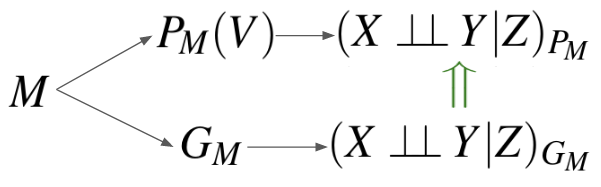
\includegraphics[width=.4\linewidth]{pics/my_own/dsep_Markov_flow.png}
\caption{When $M$ has a unique solution, the green implication is the directed global Markov property (validity of $d$-separation).}
\label{fig:dsep-Markov-flow}
\end{figure}

For an illustration of how $d$-separation may not hold for cyclic SCMs, consider the following example from \cite{Acyclification} (and further discussed in \cite{Foundations}).

\begin{example}[Counterexample: Loss of $d$-separation validity]
\label{counter}

Consider the SCM $M=(\mathbf{U},\mathbf{V},F,P(\mathbf{U}))$ with $\mathbf{u}=[u_1,u_2,u_3,u_4]\in \R^4$, $\mathbf{v}=[x_1,x_2,x_3,x_4]\in\R^4$, where $F$ is defined component-wise by
\[
f_1(\mathbf{v},\mathbf{u}) = u_1, \quad f_2(\mathbf{v},\mathbf{u}) = u_2, \quad
f_2(\mathbf{v},\mathbf{u}) = x_1x_4+u_3, \quad f_4(\mathbf{v},\mathbf{u}) = x_2x_3+u_4 
\]
and $P(\mathbf{U})$ is the standard-normal distribution on $\R^4$. The causal graph $G_M$ is shown in Figure \ref{fig:acyclification} (left). For every equilibrium of $M$, the induced observational distribution $P_M(\mathbf{V})$ satisfies $(X_1 \nCI X_2 \mid X_3,X_4)_{P_M}$.
However, $X_1$ and $X_2$ are $d$-separated given $\{X_3,X_4\}$ in the causal graph; that is, $(X_1 \CI X_2 \mid X_3,X_4)_{G_M}$. 
Hence, the global directed Markov property does not hold for $M$.
\end{example}

\begin{figure}
\centering
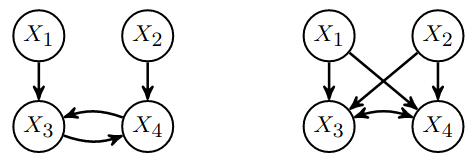
\includegraphics[width=.4\linewidth]{pics/cited/acyclification_Foundations.png}
\caption{The causal graph of Example \ref{counter} (left) and its acyclification (right). Source: \cite{Foundations}}
\label{fig:acyclification}
\end{figure}

When $d$-separation is not valid (the directed global Markov property does not hold), it may be that a weaker condition is satisfied. $\sigma$-separation is an extension of $d$-separation, which works by applying $d$-separation to the acyclification of the original graph (see Figure \ref{fig:acyclification} (right) for the acyclicification of Example \ref{counter}). $\sigma$-separation implies $d$-separation; in other words, the general directed global Markov property is weaker than the directed global Markov property. The relationship between these two Markov properties can be seen in Figure \ref{fig:inputs-outputs}.

\begin{figure}
\centering
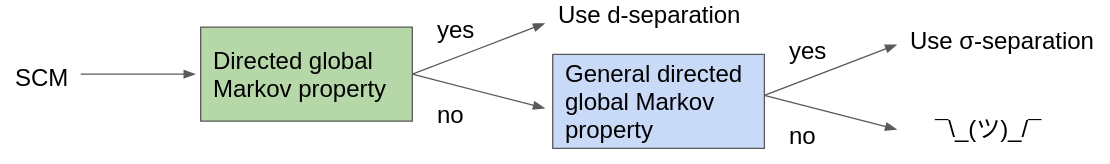
\includegraphics[width=.8\linewidth]{pics/my_own/inputs_outputs.png}
\caption{Relationship between $d$-separation and $\sigma$-separation.}
\label{fig:inputs-outputs}
\end{figure}

Acyclic SCMs, discrete SCMs (with ancestrally unique solvability), and linear SCMs (with nontrivial dependencies and positive measure) are known to satisfy the directed global Markov property \cite{MarkovCyclesLatent}. On the other hand, simple SCMs are known to satisfy the general directed global Markov property \cite{Foundations}. 

It seems reasonable that nonlinear SCMs which are asymptotically equivalent to linear SCMs should also satisfy the directed global Markov property (subject to the same restrictions of non-trivial dependencies and positive measure), and thus be able to read off conditional independencies from the graph via $d$-separation.
I conjecture that intrinsically-stable SCMs (a class of cyclic, nonlinear, continuous-domained SCMs) are precisely this class of SCMs.

\begin{problem}[Intrinsic SCMs and $d$-separation: Observational]
\label{prob:obs}

Prove whether the observational distribution of intrinsically-stable SCMs satisfy the directed global Markov property: that is, whether every conditional independence read-off by $d$-separation in the causal graph $G_M$ holds in the observational distribution $P_M(V)$.

Inputs/Outputs: Expressed by the green implication in Figure \ref{fig:dsep-Markov-flow}.
\end{problem}

(Admittedly it seems awfully convenient that a topic I studied for 4 years (undergraduate, Master's, and a bit thereafter) happens to be the right tool for the job. However, I think intrinsic SCMs can stand on their own merits):

Considered from a dynamical-systems perspective, intrinsic-SCMs have a number of promising properties relevant to causality. They have a unique equilibrium, so the potential response function of the SCM will be well-defined. They `behave’ like linear systems: they are asymptotically bounded by the dynamics of a linear system, and share the same equilibria if subject to the same forcing factor (exogenous distribution). Intuitively speaking, this means that we can go to linear-world, prove things about the system there, and the results will still hold in nonlinear-world. Furthermore, intrinsically-stable systems are quite general: they only require Lipschitz-continuity, and the domain to be a product of metric spaces (which could be something nice like $\R^4$, or something abstract like language and shapes). If a general domain like metric spaces is used, the linearization uses the metrics to map to the real numbers: in this way the domain is simplified as well.

Of particular interest for causality, intrinsically-stable systems derive their name because they are closed under a surprising number of structural transformations; that is, the resulting system will still be intrinsically-stable, and often (if applicable) the equilibria will be preserved. Some especially relevant transformations are: lengthening of paths (i.e. through time-delays \cite{ReberIntrinsic}), collapsing portions of the graph \cite{IsospectralReduction}, duplicating portions of the graph (specialization \cite{Specialization}), time-varying structural switching \cite{Switched}, and any and all isospectral transformations (transformations which preserve the eigenvalues of the system \cite{IsospectralBook}).

Given these properties of intrinsic-SCMs, a negative result for Problem \ref{prob:obs} becomes even more interesting. Since intrinsically-stable SCMs are asymptotically equivalent to linear SCMs, if $d$-separation holds for the linear but not the nonlinear SCM, this would indicate that something more than the equilibria of a cyclic SCM is needed to determine the validity of $d$-separation. 


\section{Framework Selection}

I expect to respect the framework laid out in Bongers et. al. \cite{Foundations}, which outlines a modeling framework for cyclic SCMs that is quite similar to Pearl's framework for acyclic SCMs \cite{pearl_2009}.
Cycles are incorporated simply by allowing the structural function $F$ of the SCM $M=(U,V,F,P(U))$ to be cyclic, that is, dependent on any variables in $U\cup V$.
This paper focuses on atomic interventions (which they call `perfect interventions').

There are several aspects of this framework which contrast with Pearl \cite{pearl_2009}.
The authors emphasize almost-everywhere equivalence, with respect to the observational, interventional, and counterfactual distributions, or structural functions themselves. This emphasis implicitly impacts their definitions. For example, and notably, the definition of a variable's `parents' excludes any trivial dependencies (see Appendix \ref{foundations-material}). While this definition is semantically useful (we only say there's a parent if there's a dependence that really can't be ignored) it can be slightly confusing: for example, consider the two-node linear system of $x_1 = f_1(x_1,x_2)=0.5x_1+0.1x_2$ and $x_2 = f_2(x_1,x_2)=0.1x_1+0.5x_2$. According to the definitions of \cite{Foundations}, $x_1$ and $x_2$ are both parents of each other, yet no self-cycles exist, because there exists an SCM which is asymptotically equivalent without self-cycles. (This property of linear systems is discussed further in \cite{LearningLinear}).

The primary contribution of \cite{Foundations} is in demonstrating that simple SCMs preserve many of the properties of acyclic SCMs (although notably, not $d$-separation). Simple SCMs are defined as SCMs which are uniquely solvable with respect to every subset of variables. Consequently, the observational, interventional, and counterfactual distributions exist and are unique. Furthermore, simple SCMs satisfy the general directed global Markov property; are closed under marginalization; and the causal semantics of the causal diagram's subgraph match the structure of the submodel of the SCM.
% The relationship of simple SCMs to previous classes of cyclic SCMs explored in the literature is shown in Figure \ref{fig:set-inclusion}.

\begin{remark}[Relation of Intrinsic SCMs to Previous Literature]
I conjecture that intrinsic SCMs are a subset of simple SCMs (specifically, this claim implies that intrinsic SCMs are uniquely solvable with respect to every subset of variables). Acyclic SCMs can, in a trivial way, be expressed as intrinsic SCMs, so long as we tweak the definition of intrinsic SCMs slightly to allow for unbounded Lipschitz constants, but which don't affect the spectrum of the corresponding linear SCM $\mathcal{L}(M)$. Two points are worth highlighting from this conjectured set inclusion (Figure \ref{fig:set-inclusion}). Firstly, while broad in many ways, intrinsic SCMs are still a very restrictive class. Secondly, many interesting linear cyclic SCMs will not be intrinsically stable (for instance, the well-studied supply and demand example from e.g. \cite{SupplyDemand}), just as many linear SCMs aren't acyclic \cite{LearningLinear}, nor simple \cite{Foundations}.
\end{remark}

\begin{figure}
\centering

\includegraphics[width=.6\linewidth]{pics/my_own/set_inclusion.png}
\caption{Conjectured set-inclusion relation of the class of intrinsically-stable SCMs relative to other classes of cyclic SCMs. Based on \cite{Foundations}}
\label{fig:set-inclusion}
\end{figure}

Settable systems are an alternative framework for cyclic causality \cite{White&Chalak} which I considered using, as it has proven insightful for game theory \cite{GameIncomplete}. The primary strength of settable systems lies in its convenient treatment of multiple equilibria. However, since intrinsic SCMs do not have multiple equilibria, this is more functionality than is needed right now. Settable systems also rely on fairly low-level representations of the optimization pressure on the equilibria (for example, to select one equilibria from many) \cite{CausalGames}, and are less closely related to the acyclic SCM framework introduced during last semester.

\section{Preliminary Results}

\subsection{Numerics}

\begin{figure}
\centering
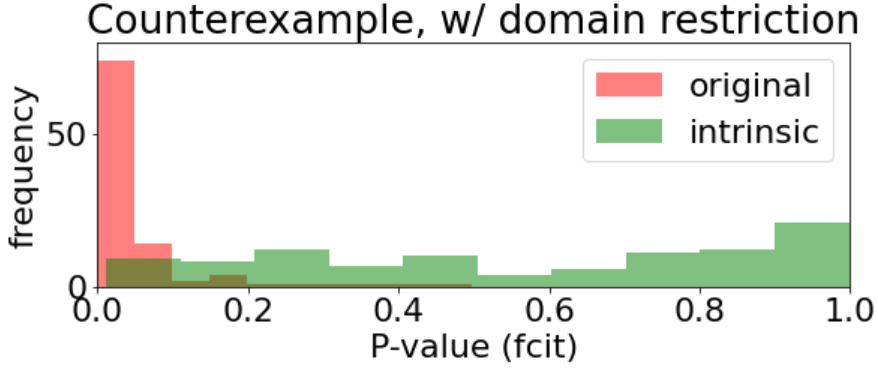
\includegraphics[width=.5\linewidth]{pics/my_own/counterexample_domain_restriction.png}
\caption{The counterexample discussed in \cite{Acyclification,Foundations}. Here, conditional independence is tested while restricting the exogenous variables to be drawn from a truncated multivariate normal distribution (such that the SCM as a whole is intrinsically stable). The conditional independence identified by $d$-separation is now present in the observational distribution.}
\label{fig:counterexample_domain_restriction}
\end{figure}

Consider again Example \ref{counter}, the counterexample popular in the literature. If we restrict the domain of the exogenous variables to $\mathbf{u}=\in [-0.5,0.5]^4$ (which we may do by discarding any samples outside of this range), the resulting SCM is intrinsically-stable. Hence, if Problem \ref{prob:obs} resolves in the affirmative, we should observe that the observational distribution of the restricted-domain SCM should have the conditional independence of $(X_1 \CI X_2 \mid X_3,X_4)_{P_M}$, matching the independence $(X_1 \CI X_2 \mid X_3,X_4)_{G_M}$ computed by $d$-separation from the graph.

The results of this test are shown in Figure \ref{fig:counterexample_domain_restriction}. In order to test the conditional independence numerically over a continuous domain, the python package \verb|fcit| \cite{fcit} was used. The resulting p-values are distributed roughly uniformly on $[0,1]$, consistent with an \verb|fcit| result of conditional independence.
 
\subsection{Proof sketch for Problem \ref{prob:obs}}

\begin{figure}
\centering
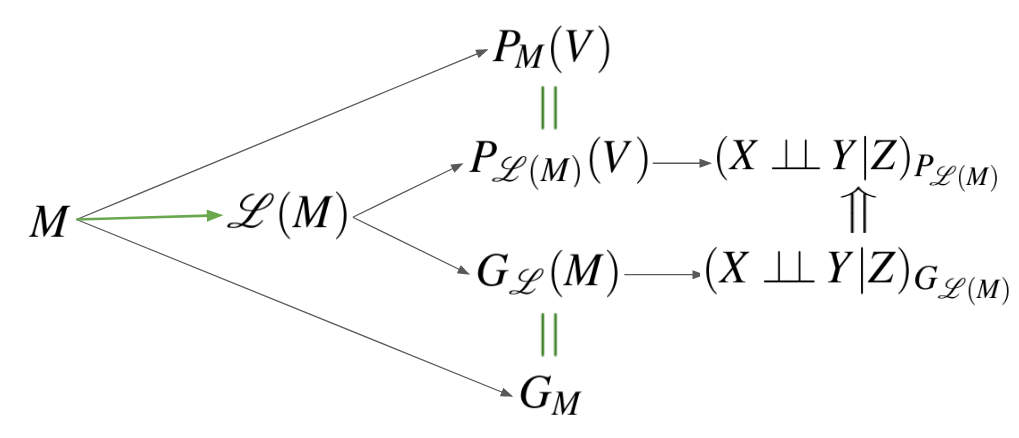
\includegraphics[width=.5\linewidth]{pics/my_own/research_plan_flow.png}
\caption{Conjectured proof sketch, for positive resolution of Problem \ref{prob:obs}.}
\label{fig:research-plan-flow}
\end{figure}

\begin{figure}
\centering
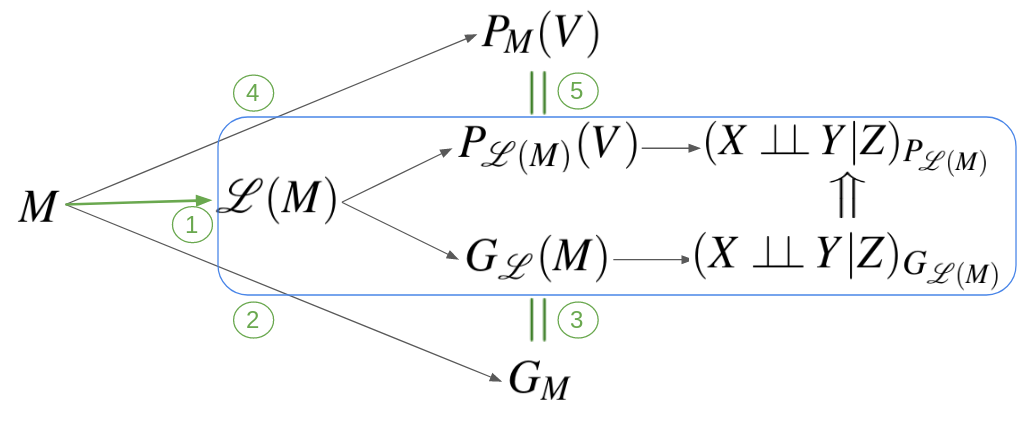
\includegraphics[width=.5\linewidth]{pics/my_own/research_plan_numbered_boxed.png}
\caption{Identical as Figure \ref{fig:research-plan-flow}, but with helpful labels of the conjectured relations. Note that the portion contained within the blue box simply expresses that the associated linear SCM $\mathcal{L}(M)$ satisfies the directed global Markov property (Figure \ref{fig:dsep-Markov-flow}).}
\label{fig:research_plan_numbered_boxed}
\end{figure}

My research strategy for proving the affirmative of Problem \ref{prob:obs}, comprises of two parts (see Figure \ref{fig:research-plan-flow}): First, relate $M$ to a linear SCM $\mathcal{L}(M)$ which satisfies the directed global Markov property. Secondly, show that $M$ and $\mathcal{L}(M)$ respect the same graph and are observationally equivalent.

This can be broken down into greater detail via Figure \ref{fig:research_plan_numbered_boxed}. Each of these lemmata (with a rough proof sketch) are described below:

\begin{enumerate}
  \item $M\rightarrow \mathcal{L}(M)$: Show that for every intrinsically-stable $M$, there exists a linear SCM $\mathcal{L}(M)$ which satisfies the directed global Markov property (the blue box).
  \item $M\rightarrow G_M$: Always possible by definition, I believe.
  \item $G_M = G_{\mathcal{L}(M)}$: Show that for every node, the parents are preserved (according to \cite{Foundations}'s definition of parents: see Appendix \ref{foundations-material}).
  \item $M \rightarrow P_M(V)$: Show that if $M$ is intrinsically stable, it is uniquely solvable.
  \item $P_M(V) = P_{\mathcal{L}(M)}(V)$: Translate intrinsic-stability property of $M$ and $\mathcal{L}(M)$ have the same equilibrium solutions, to SCMs. Show that this means they induce the same observational distributions.
\end{enumerate}

\section{Future Possibilities}
\subsection{Anticipated Implications}

I consider it is worth checking early in one's research whether hypothetical success would itself be ludicrous, even if this means initially high exposure to unverified speculation.
To keep this report appropriately rigorous, however, my speculation about these potential implications is located in Appendix \ref{speculation}. In brief:

\begin{enumerate}
  \item Should Problem \ref{prob:obs} resolve positively, I expect that nonlinear intrinsic SCMs $M$ will be counterfactually equivalent to their linearizations $\mathcal{L}(M)$ (and thus inherit nearly all of their nice properties).
  \item This would not violate the `No Free Lunch' Principle: $\mathcal{L}(M)$ will be no easier to use for modeling purposes.
\end{enumerate}

\subsection{Potential (future) Collaborators}

I recently met with both Lewis Hammond (Oxford) and Christian Kroer (Columbia, IOER department). Both are very interested in `game theory + causality', which I find the most compelling motivator for cyclic causality research. To the extent that nonlinear, cyclic SCMs are `locally intrinsic' (as Example \ref{counter} was shown to be here) there may be some valuable collaborations to be had. For now, I'll just keep occasional dialogue with them to see what arises.


% pdflatex main
% bibtex main
% pdflatex main
% pdflatex main

\bibliographystyle{plain}
\bibliography{refs}

\section{Appendix: Musings Beyond Observational $d$-separation}

\subsection{$d$-separation and Interventional Distributions} \label{speculation}

I’m very confident that the space of intrinsic SCMs is closed under interventions (if you intervene on an intrinsic SCM, the resulting SCM is also intrinsic).
I’m also confident that the operations of atomic intervention $M\rightarrow M_x$ and linearization $M\rightarrow \mathcal{L}(M)$ commute for intrinsic SCMs.
Thus, if Problem \ref{prob:obs} resolves in the affirmative, I conjecture it should be straightforward to demonstrate (atomic) interventional equivalence between a nonlinear, intrinsic SCM and its associated linear SCM $\mathcal{L}(M)$.

\begin{problem}[Intrinsic SCMs and $d$-separation: Interventional]
\label{prob:int}

Prove whether the interventional distribution of intrinsically-stable SCMs satisfy the directed global Markov property: that is, whether every conditional independence read-off by $d$-separation in the causal graph $(G_M)_{\overline{X}}$ holds in the interventional distribution $P_{M_x}(V)$.
\end{problem}

Note the order of operations for $(G_M)_{\overline{X}}$: first we generate the causal graph of $M$, then intervene with an atomic intervention on that graph. This is in contrast to $P_{M_x}(V)$, where we first perform an atomic structural intervention on $M$, then generate the distribution of this new SCM.

If Problem \ref{prob:int} answers in the affirmative, I believe it follows that the do-calculus is valid for intrinsic SCMs.

\subsection{$d$-separation and Counterfactual distributions}

I also confidently conjecture that (if Problem \ref{prob:obs} resolves positively) intrinsic SCMs are also closed under the “mirror” transformation.
(The mirror operation is useful for defining cyclic counterfactuals: you construct a `twin SCM' using the twin network method). 
This operation, if I understand correctly, should merely reduce to the duplication of a strongly connected component, but otherwise leave strongly connected components unchanged. Since intrinsic-stability is based on a spectral criteria, one can without loss of generality simply consider each strongly connected component of the system independently. (Indeed, almost all my remaining uncertainty derives from wondering whether I've missed some subtle-yet-crucial detail in the definitions of cyclic SCMs).

\begin{problem}[Intrinsic SCMs and $d$-separation: Counterfactual]
\label{prob:count}

Prove whether the counterfactual distribution of intrinsically-stable SCMs satisfy the directed global Markov property: that is, whether every conditional independence read-off by $d$-separation in the twin network holds in the corresponding counterfactual distribution of the twin SCM.
\end{problem}

If Problem \ref{prob:count} resolves positively, then this would mean that the $M$ and $\mathcal{L}(M)$ are not merely observationally or interventionally equivalent, but \emph{counterfactually equivalent}. (However, they are precluded from being \emph{structurally equivalent} according to the definition in \cite{Foundations}, since this requires not only almost-everywhere equivalence of equilibrium solutions, but of the transition functions themselves.)

I do not expect this counterfactual equivalence (should it actually hold) to violate the `No Free Lunch' principle.
The counterfactual equivalence of an intrinsic SCM $M$ with a linear SCM $\mathcal{L}(M)$ may do little more than imply that nice properties (like $d$-separation) are valid for $M$, as far as modeling is concerned, because I expect that the complexity of $F_M$'s nonlinearity simply gets pushed into the linear SCM's exogenous distribution $P_{\mathcal{L}(M)}(U)$.

\section{Appendix: Relevant Definitions for Cyclic SCMs}\label{foundations-material}
The following definitions are copied verbatim from \cite{Foundations}, and provided here only for ease of reference. Consequently they differ somewhat from the notation of this report.

\centering
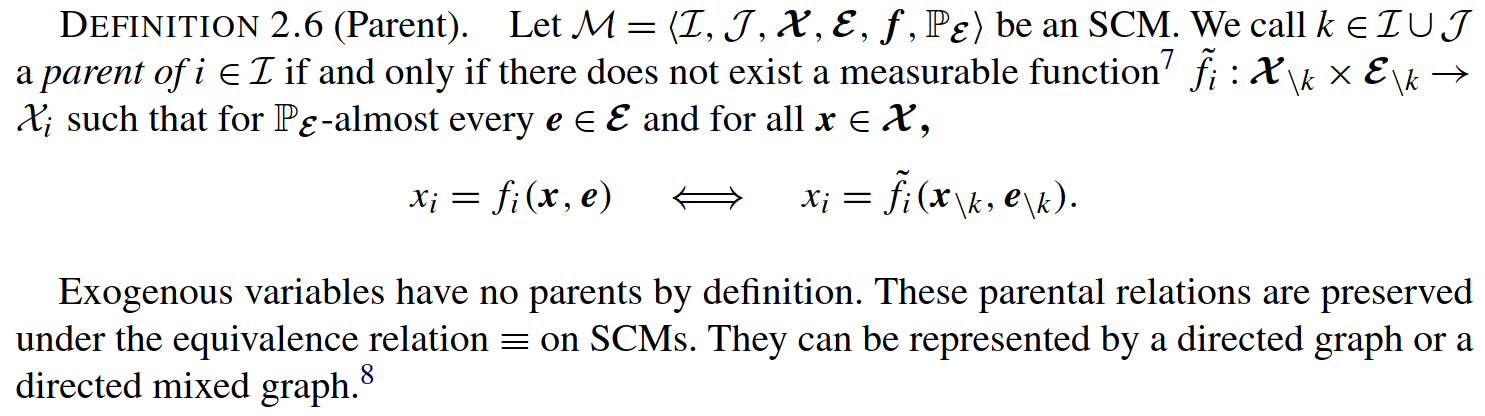
\includegraphics[width=.8\linewidth]{pics/cited/parents_Foundations.png}

\centering
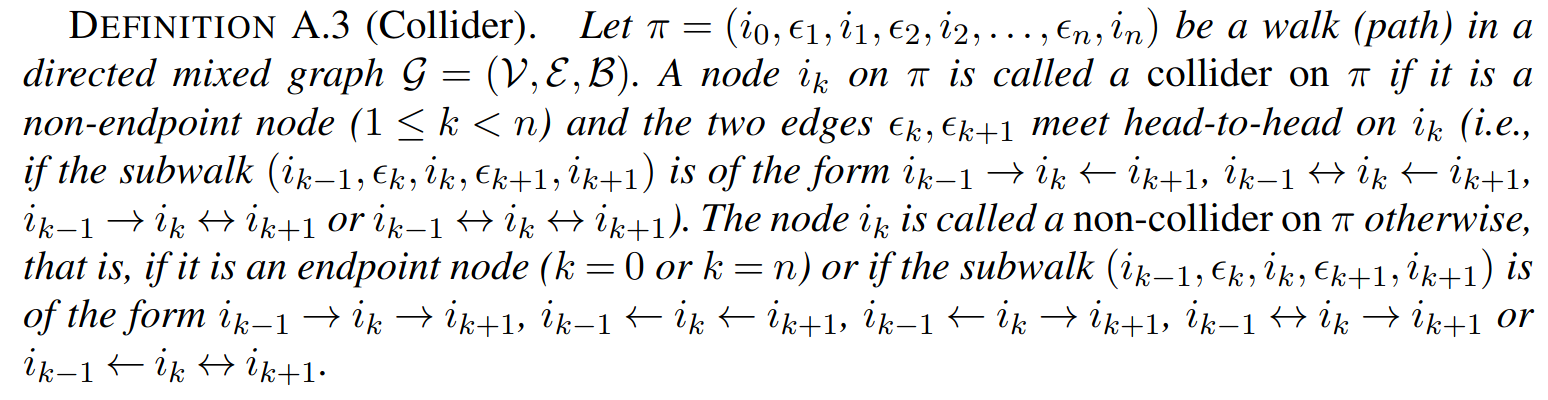
\includegraphics[width=.8\linewidth]{pics/cited/collider_Foundations.png}

\centering
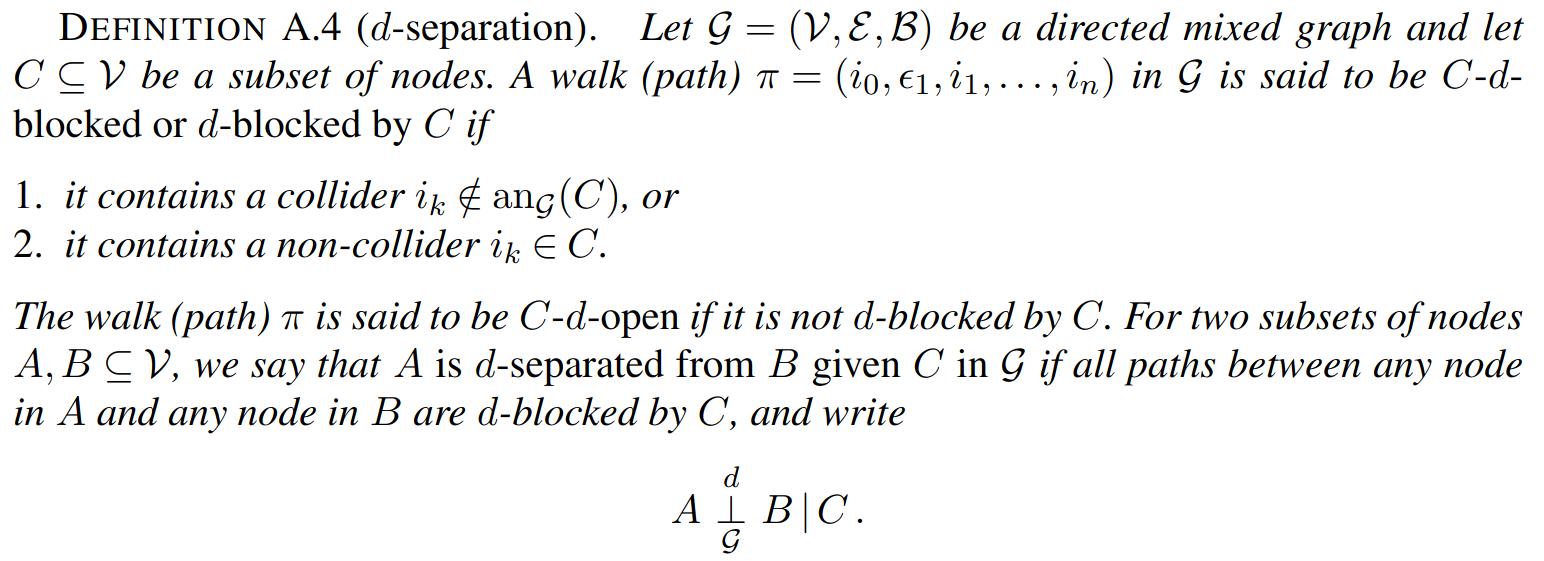
\includegraphics[width=.8\linewidth]{pics/cited/d-separation_Foundations.png}

\centering
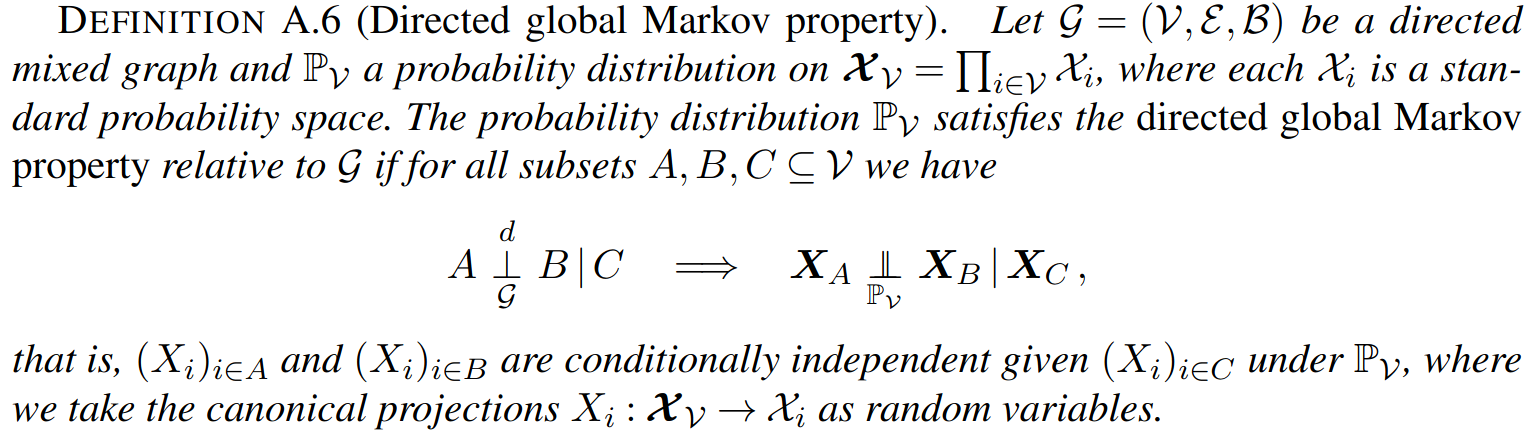
\includegraphics[width=.8\linewidth]{pics/cited/directed_global_Markov_Foundations.png}

\end{document}
